\section{Problems Remaining in OpenIE}

    After addressing multiple key issues of OpenIE systems through \shortname, we sought to analyse the problems that are still prevalent with OpenIE systems. To begin with, we carefully analysed the erroneous outputs of \shortname\ and other systems. We could broadly categorise the remaining errors into the following types.

    \subsection{Missing Information}
        The major source of OpenIE errors is missing information in the OpenIE tuples. For \shortname, about 66\% of the sentences have at least one of the relations or arguments or both missing in predicted extractions, which are present in gold extractions. This leads to incomplete information. For eg.

        \begin{verbatim}
            Sentence:
            ``George got married to Alice in March beside the lake.''
            Set of Extractions with Missing Information:
            ( George ; got married ; )
            Gold Extractions:
            ( George ; got married to ; Alice )
            ( George ; got married in ; March )
            ( George ; got married beside ; the lake )
        \end{verbatim}

    \subsection{Incorrect Conjunction Splitting}

        One the guidelines of OpenIE is \emph{atomicity}. The principle of atomicity states that every tuple must be indivisible. In case of sentences with conjunctions, this translates to deriving multiple OpenIE tuples from the sentence, one with each conjunct. The output tuples where the coordination phrase has not been split are counted under the category of incorrect conjunction splitting. For eg.

        \begin{verbatim}
            Sentence:
            ``I ate an apple and an orange.''
            Incorrect Extraction:
            ( I ; ate ; an apple and an orange )
            Gold Extractions:
            ( I ; ate ; an apple )
            ( I ; ate ; an orange )
        \end{verbatim}
        
        It is worth noting that as much as 32\% of \shortname's errors are attributed to incorrect conjunction splitting.

    \subsection{Grammatical Errors}

        OpenIE tuples should not only identify the different parts of an extraction correctly, but should also lay them down in a grammatical structure. This means that when the extraction is serialised, the yielded sentence should be grammatical. For eg.

        \begin{verbatim}
            Sentence:
            ``US President Donald Trump''
            Incorrect Extraction:
            ( Donald Trump ; President ; US )
            Gold Extractions:
            ( Donald Trump ; is the president of ; US )
        \end{verbatim}

        Roughly 38\% of \shortname's errors were due to grammatical erros in its extractions.

    \subsection{Missing Output Context}

        OpenIE systems should be capable of generating the context of the output tuples whenever necessary. Rule-based systems like OpenIE-5 were able to generate context alongside the extractions yet \shortname\ and many recent OpenIE systems do not possess this ability. For eg.

        \begin{verbatim}
            Sentence:
            ``The police claimed, "Brutus broke into the house." ''
            Incorrect Extraction:
            ( Brutus ; broke into ; the house )
            Gold Extractions:
            [Context: The police claimed] ( Brutus ; broke into ; the house )
        \end{verbatim}

    \subsection{Coreference Resolution}

        OpenIE systems should be able to resolve coreferences in the sentence. They should generate each tuple such that the tuples do not depend on each other to clarify the their meaning. However, most OpenIE systems are not able to resolve coreferences till data. For eg.

        \begin{verbatim}
            Sentence:
            ``Alice ate an apple and then she went for a walk.''
            Incorrect Extraction:
            ( she ; went for ; a walk )
            Gold Extractions:
            ( Alice ; went for ; a walk )
        \end{verbatim}

    \subsection{Incorrect Identification of Boundaries}

        OpenIE systems are also known to incorrectly identify the relation and argument boundaries within a sentence. This includes errors like the object argument starts with a preposition instead of placing that preposition within the relation. In case of \shortname, nearly 60\% of the sentences have the separator between relation and argument identified at the wrong place. The major cause of this type of error is attributed to fallacies in the training data, however it may even creep in otherwise. For eg.

        \begin{verbatim}
            Sentence:
            ``Jonathon is going for a walk.''
            Incorrect Extraction:
            ( Jonathon ; is going ; for a walk )
            Gold Extractions:
            ( Jonathon ; is going for ; a walk )
        \end{verbatim}

\section{Why to Split Conjunctions?}

    OpenIE systems perform much better on short simple sentence as compared to long and complicated ones. This seems obvious since long sentences encompass multiple informations often intertwined in complex sentence structures. It requires much more expertise even for a human annotator to pick out all of them in the form of OpenIE tuples. However, when viewed in light of incorrect conjunction splitting done by OpenIE systems, this gives rise to a potent idea. We could design a separate module to explicitly break a complex sentence into several simple ones by splitting on conjunctions. Passing these simpler sentences through OpenIE systems inplace of the original sentence would yield higher quality extractions. This seemed to be a low-hanging fruit, hence we decided to go ahead with this idea.

    \subsection{Analysis of Existing Systems}
        In order to validate our hypothesis that a better module for conjunction splitting was actually required, we analysed the conjunction splitting ability of some popular rule-based systems. A separate analysis had shown that \verb|and| is the most frequent conjunction occuring in sentences with conjunctions. Hence, in order to expidite the current analysis, we chose only sentences with and. There were about 285 of them in the CaRB dev set. We manually annotated (refer table \ref{tab:conj_split_systems}) each of these sentences to determine how many of them were distributive i.e. how many sentences were such that they could be split into multiple simpler sentences.

        % TABLE: Conjunction Splitting Systems
        \begin{table*}[h]
            \centering
            \resizebox{0.5\textwidth}{!}{%
            \begin{tabular}{|c|c|c|c|}
            \hline
            \textbf{System} &
            \textbf{\begin{tabular}[c]{@{}c@{}}No. of\\ Sentences\\ with AND\end{tabular}} &
            \textbf{\begin{tabular}[c]{@{}c@{}}No. of\\ Distributive\\ Sentences\end{tabular}} &
            \textbf{\begin{tabular}[c]{@{}c@{}}Percentage of\\ Distributive\\ Sentences\end{tabular}} \\ \hline
            Gold     &     & 207 & 72.6 \\ \cline{1-1} \cline{3-4} 
            OpenIE-4 & 285 & 130 & 45.6 \\ \cline{1-1} \cline{3-4} 
            OpenIE-5 &     & 261 & 91.5 \\ \hline
            \end{tabular}%
            }
            \caption{Conjunction Splitting in Existing Rule-Based Systems}
            \label{tab:conj_split_systems}
        \end{table*}

        Of the 285 sentences annotated, 72.6\% were distributive. OpenIE-4 and OpenIE-5, two popular rule-based systems used for this analysis, split up 45.6\% and 91.5\% of these sentences respectively. This confirms that OpenIE-4 is too conservative in splitting conjunctions whereas OpenIE-5 is too aggressive. Moreover, none of them is close enough to the ideal split ratio of about 72\%. This analysis, therefore, confirms our hypothosis that a better module for conjunction splitting is required.

\section{HC-Tree Based Splitting}

    In this section, we discuss an approach for a conjunction-splitting model. The idea is based on \textbf{Hierarchical Coordination Trees}. An HC tree is an efficient representation of nested coordination phrases occuring in a sentence. Figure \ref{fig:hc_tree_eg} depicts an example of a complex sentence with nested coordination phrases and the corresponding HC tree.

    % HC Tree example
    \begin{figure*}[h]
        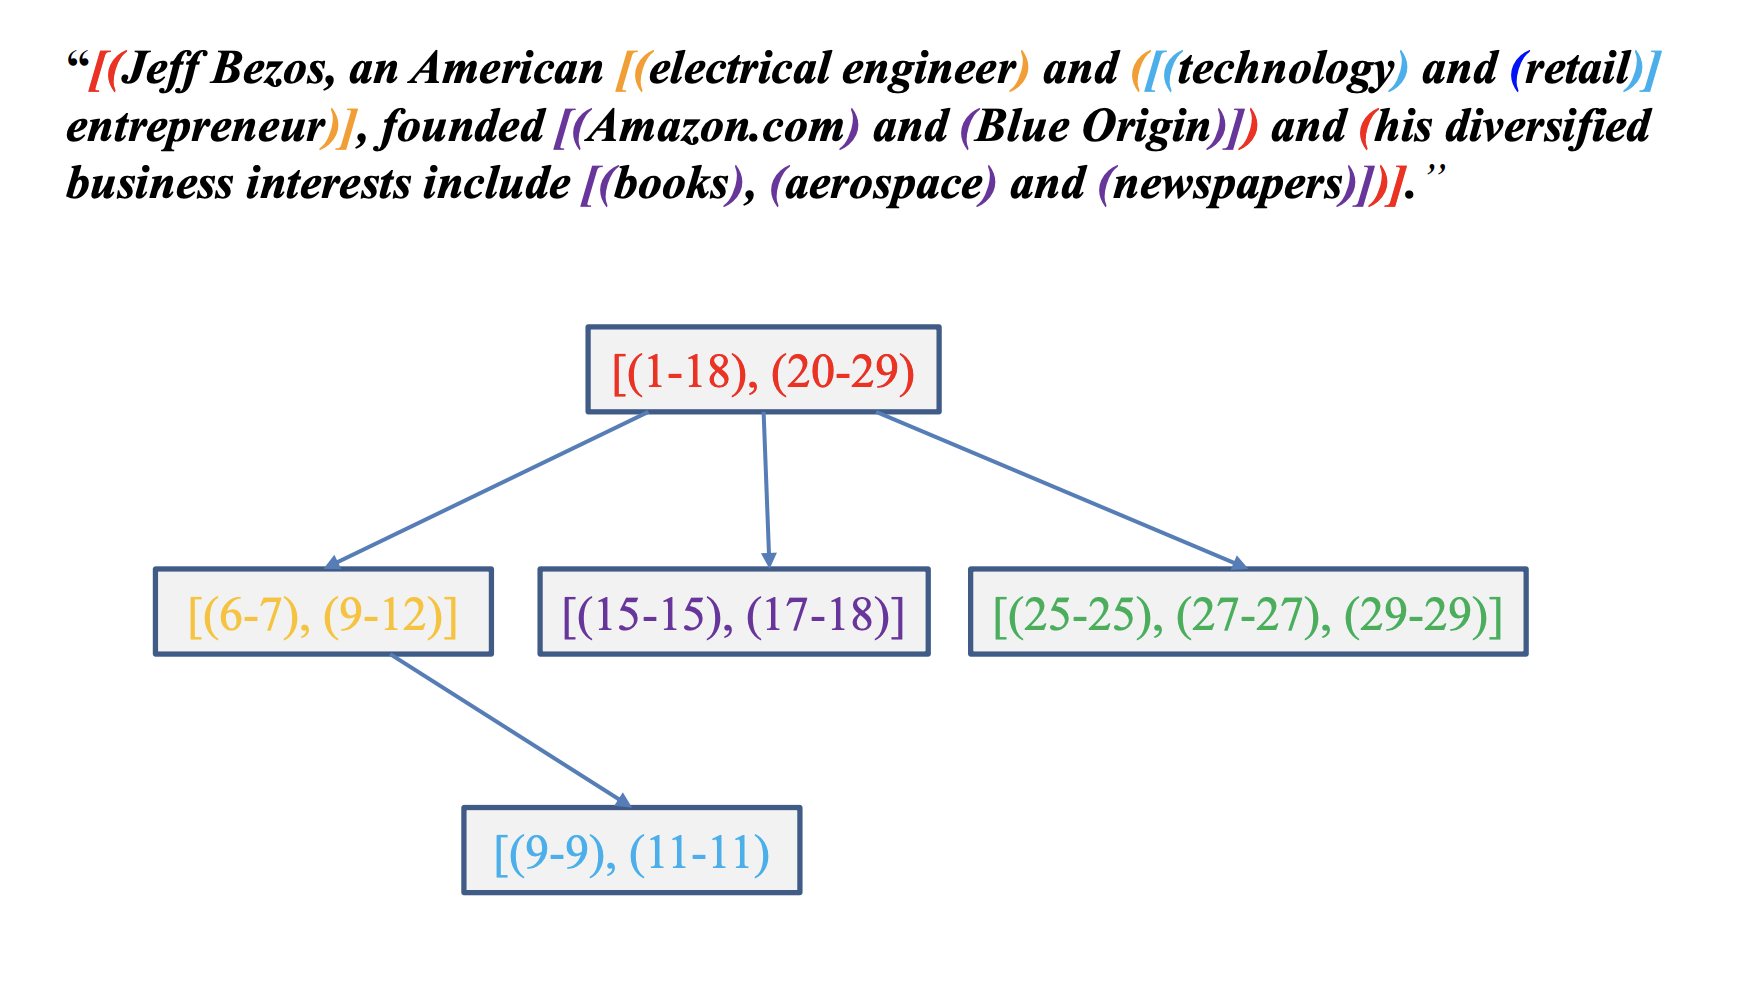
\includegraphics[width=.99\hsize]{images/hc_tree.png}
        \caption{Example of a sentence and its Hierarchical Coordination (HC) Tree}
        \label{fig:hc_tree_eg}
    \end{figure*}

    For our analysis, we use $[D_{i}]$ token at the beginning and end of each coordination phrase. Also, each conjunct is encapsulated with $[SS]$ and $[ES]$ tokens.

    \subsection{Properties of Conjuncts}
        It is important to discuss two key properties of conjuncts before diving into the approach. Consider the sentence \verb|I ate [D1] [SS] an apple [ES] and [SS] an orange [ES] [D1].| to understand the properties.
        \begin{enumerate}
            \item \textbf{Similarity:} The conjuncts are similar to each other in their syntactic form.
            
            For eg., \verb|an apple| and \verb|an orange| are syntactically similar.

            \item \textbf{Replaceability:} Each of the conjunct can potentially replace the entire coordination phrase in the original sentence and to yield a meaning sentence.
            
            For eg. \verb|``I ate an apple.''| and \verb|``I ate an orange.''| are both meaningful sentences.
            
        \end{enumerate}

    \subsection{Proposed Approach}

        \subsubsection{Step 1: Generation of HC Tree}
        
            First of all, we need to generate an HC tree for the given sentence. For this purpose, we use a sequence to sequence model with BERT as encoder and a Tree-Based decoder \citep{wang&al18}. We use data from PennTree Bank \citep{PennTreeBank} dataset due to the following reasons:
            \begin{enumerate}
                \item \textit{Sufficient number of sentences:} The PennTree Bank has a dev and test set of 1700 and 2416 sentences respectively.
                \item \textit{Contains coordinations upto depth 3:} PennTree Bank also has a significant number of sentences with coordinations nested at depths upto 3. It contains 756, 87 and 5 sentences with conjunctions at depth 1, 2 and 3 respectively in dev set.
                \item \textit{Resembling Fraction of Distributive Conjunctions:} The fraction of sentences that are distributive are similar for PennTree Bank (64.5\%) and the CaRB gold dataset (72.6\%) (refer to table \ref{tab:conj_split_systems}). This indicates that the distribution of sentences in the PennTree bank is similar to that found in a general corpus.
            \end{enumerate}

        \subsubsection{Step 2: Obtaining Split Sentences from HC Tree}

            The next step is to split the original sentence and obtain simpler sentences. This is done in an iterative manner with increasing depths of split. At each depth, we replace each coordination phrase with all the conjuncts one-by-one. Then for each of the simpler sentences obtained, we repeat this procedure at the next depth till the sentence contains no more coordination phrase. For eg.

            \begin{verbatim}
Input - Premise (HC tree) :
Today, [D1] [SS] Ram [ES] and [SS] Shyam [ES] [D1] ate [D1] [SS] an apple
 [ES] and [SS] an orange [ES] [D1] .

Output - Hypothesis (simple sentences) :
Today, Ram ate an apple .
Today, Ram ate an orange .
Today, Shyam ate an apple .
Today, Shyam ate an orange .
            \end{verbatim}

        \subsubsection{Step 3: Validation of Hypothesis}

            In this step, we check whether or not the coordination phrase split at step 2 was actually distributive. Consider the following examples of a distributive and non-distributive sentence.
            
            \begin{verbatim}
Example: Distributive Sentence
PaineWebber Inc. [D1] [SS] filmed a new television commercial at 4 p.m. EDT
 yesterday [ES] and [SS] had it on the air by last night [ES] [D1]  .

PaineWebber Inc. filmed a new television commercial at 4 p.m. EDT yesterday .
PaineWebber Inc. had it on the air by last night .

Example: Non-Distributive Sentence
The [D1] [SS] Ways [ES] and [SS] Means [ES] [D1]  Committee will hold a
 hearing on the bill next Tuesday .

The Ways Committee will hold a hearing on the bill next Tuesday .
The Means Committee will hold a hearing on the bill next Tuesday .
            \end{verbatim}

            We use pretrained FastText vectors (trained on Wikipedia and Common Crawl datasets) to encode:
            \begin{itemize}
                \item The Premise i.e. the original complex sentence
                \item The Hypothesis i.e. all the simple sentences obtained after splitting
                \item General Sentence Corpus (we use 3.9M sentences from Wikipedia of which 700K sentences contain conjunctions)
            \end{itemize}

            Next, we compare the \emph{Cosine Similarity score} of the encoded premise and hypothesis with the encoded sentences of the corpus. The similarity-score of these sentences with the general sentences is treated as a proxy for the probability of encountering such a sentence in a general corpus. If the similarity-score of the premise is higher than the least among all similarity-scores of the hypothesis, then we ignore the split and use the premise as it is. Else, we use the split sentences.

            Note that steps 2 and 3 have to be done in succession for each depth. This means, that we will split (step 2) the coordination phrases at depth 1, then verify (step 3) each split. Only after that will we move towards splitting (step 2) at depth 2.

        \subsubsection{Step 4: Feeding the sentence to \shortname}

            By the time we reach this step, we would have split all distributive sentences and idenfied simpler sentences had they existed. This is the final step wherein we simply feed these sentences to an OpenIE system, \shortname\ in our case. For eg.

            \begin{verbatim}
Input to IMoJIE, previously :
In these locations , Mr. Friedman says , Retailers are increasingly cautious
about expanding and rents have remained steady or in some cases have declined .

Input to IMoJIE, now :
In these locations , Mr. Friedman says , Retailers are increasingly cautious
about expanding .
In these locations , Mr. Friedman says , rents have remained steady .
In these locations , Mr. Friedman says , rents in some cases have declined .
            \end{verbatim}

    \subsection{Drawbacks}

        The approach seems promising, however it has several drawbacks.
        \begin{enumerate}
            \item \emph{Sentences closer in encoded space are not semantically similar}
            The example below demonstrates the top two sentences from the general corpus that are most similar to the given sentence. Clearly, the retrieved sentences are not particularly similar.

            \begin{verbatim}
Joe Russo (musician) ( born December 18 , 1976 ) is an American drummer
 and half of the Benevento/Russo Duo .
0.957    Tiffany Shepis ( born September 11 , 1979 ) is an American
actress from New York City , who has been involved in film-making 
since the age of 12 .
0.956    Vincent Grier ( born March 14 , 1983 ) is an American former 
college basketball player for the University of Minnesota Golden Gophers .
            \end{verbatim}
            
            \item \emph{Lack of standard metric to decide extent of similarity of sentences}
            
            The absence of any standard metric to quantify similarity of sentences makes it difficult to comment on the degree of similarity of the retrieved sentences.

            \item \emph{Cosine similarity is not representative}
            
            The aim of fetching similar sentences is to calculate a proxy for the probability of the coordination phrase appearing in the context of the sentence i.e. \\Prob(coordination phrase | context of the sentence). However, we find that \emph{cosine similarity score} is not representative of the likelihood of the encoded sentence occuring in a general sentence corpus. There are two main reasons for this:
            \begin{itemize}
                \item Cosine similarity is high even for non-similar sentences. As evident from the previous example, the cosine similarity for the best matching sentences were more than 0.95 even though the sentences did not appear to be similar.
                
                \item It does not vary much for top few matches. For most of the sentences, the best similarity scores where around 0.95, which is counter intuitive since this indicates that all sentences are almost equally likely to appear in the general corpus. This is trivially false.
            \end{itemize}
            
        \end{enumerate}

        On these grounds, we digress away from the HC-Tree based approach to conjunction splitting. We move towards rule-based systems for conjunction splitting.

\section{Patterns dictating Distributivity of Coordination Phrase}

    In order to develop a better understanding of distributivity of coordination phrases, we identify the patterns and sentence structures that ultimately dictate whether a sentence will be distributive or not. We notice that any coordination phrase can be matched to a logical operator that it. In our description of the observed patterns, we capitalise the logical operators to distinguish them from similarly spelled conjunctions. Following are the rules that we came up with.
    \begin{itemize}
        \item XOR can never be split
        
        \item BUT behaves similar to AND in most cases, it is just that the intonation is different
        
        \item OR cannot be split in the consequent. For eg.
            \begin{verbatim}
    If X happens, then Y or Z will happen.
    Incorrect to split as:
        If X happens, then Y will happen.
        If X happens, then Z will happen.
            \end{verbatim}

        \item OR can be split in the anticedent. For eg.
            \begin{verbatim}
    If X or Y happen, then Z will happen.
    Correct to split as:
        If X happens, then Z will happen.
        If Y happens, then Z will happen.
            \end{verbatim}
        
        \item AND cannot be split in the antecedent. For eg.
        \begin{verbatim}
    If X and Y happen, then Z will happen.
    Incorrect to split as:
        If X happens, then Z will happen.
        If Y happens, then Z will happen.
        \end{verbatim}

        \item AND can be split in the consequent. For eg.
        \begin{verbatim}
    If X happens, then Y and Z will happen.
    Correct to split as:
        If X happens, then Y will happen.
        If X happens, then Z will happen.
        \end{verbatim}
        
        \item Sequential Constructs ($A \rightarrow B \rightarrow C$) cannot be split. For eg.
        \begin{verbatim}
Mr. Farley followed a similar pattern when he acquired Northwest 
Industries Inc. and then sold much of its assets.
        \end{verbatim}
        
    \end{itemize}

\section{Analysis of Non-Distributive Sentences}

    We also manually annotated about 220 sentences to identify reasons that lead to non-distributivity of sentences. Of these 220 sentences, 39 were found to be non-distributive due to the reasons listed below. Table \ref{tab:non_dist_reasons} shows the significance of the various reasons for non-distributivity of sentences.

    \begin{table*}[h]
        \centering
        \resizebox{0.5\textwidth}{!}{%
        \begin{tabular}{|c|c|}
        \hline
        \textbf{Reason}            & \textbf{Significance} \\ \hline
        Unsplittable Entity        & 38.5\%                \\ \hline
        Relation forbids Splitting & 25.6\%                \\ \hline
        Antecedent AND             & 15.4\%                \\ \hline
        Between construct          & 7.7\%                 \\ \hline
        Either-Or construct        & 2.6\%                 \\ \hline
        Consequent OR              & 2.6\%                 \\ \hline
        Idiomatic Phrase           & 2.6\%                 \\ \hline
        BUT changes meaning        & 2.6\%                 \\ \hline
        Sequential construct       & 2.6\%                 \\ \hline
        \end{tabular}%
        }
        \caption{Reasons for non-distributivity of sentences along with their significance based on the frequency of occurence}
        \label{tab:non_dist_reasons}
    \end{table*}

    \begin{itemize}
        \item \textbf{Unsplittable Entity:} When an entity is being referred to in the conjuncts and it cannot be divided. For eg.
        \begin{verbatim}
[D1] [SS] Ways [ES] and [SS] Means [ES] [D1]  Committee
[D1] [SS] green [ES] and [SS] gold [ES] [D1] 
[D1] [SS] a run [ES] and [SS] four hits [ES] [D1]
        \end{verbatim}
        
        \item \textbf{Relation forbids splitting:} When the relation is such that splitting the sentence leads to meaningless conjuncts. For eg.
        \begin{verbatim}
In the aftermath of the 1987 debacle , the brokerage firm began
taping commercials in-house , ultimately getting its timing down
fast enough to [D1] [SS] tape a commercial after the market closed
[ES] and [SS] rush it on the air that night [ES] [D1]  .

We 're saying the worst thing that anyone can do is to see the market
[D1] [SS] go down [ES] and [SS] dump everything [ES] [D1]  , which
just drives the prices down further , says John Lampe , 
PaineWebber's director of advertising .

The team that dumped runs by the bushel on the Chicago Cubs in 
the National League playoffs was held to just one in two games by 
the home-team Oakland A 's , the gang that had been done unto 
similarly by [D1] [SS] the Los Angeles Dodgers [ES] and [SS] Orel
Hershiser [ES] [D1]  in last year 's tournament .

I [D1] [SS] 'm for the Giants today [ES] , but [SS] only because 
they lost yesterday [ES] [D1].            
        \end{verbatim}

        \item \textbf{Antecedent AND:} For eg.
        \begin{verbatim}
If you [D1] [SS] get your pitch [ES] , and [SS] take a good swing 
[ES] [D1]  , anything can happen , he later remarked .

The collapsed plan to acquire UAL Corp. , parent of United Airlines, 
spurred quick action on the legislation , [D1] [SS] introduced 
Wednesday [ES] and [SS] approved by the subcommittee on a voice vote 
yesterday [ES] [D1].

NCR said revenue declined both [D1] [SS] in the U.S. [ES] and [SS]
overseas [ES] [D1]  , reflecting a world-wide softening of the 
computer markets.
        \end{verbatim}

        \item \textbf{Between construct:} When the two conjuncts are related by \emph{between}, they cannot make meaningful sentences individually. For eg.
        \begin{verbatim}
In a possible prelude to the resumption of talks between [D1] [SS] 
Boeing Co. [ES] and [SS] striking Machinists union members [ES] [D1],
a federal mediator said representatives of the two sides will meet 
with him tomorrow .

Differences remained between the [D1] [SS] North [ES] and [SS] 
South [ES] [D1]  Korean governments , however , over conditions for 
the exchanges .

[D1] [SS] Seoul [ES] and [SS] Pyongyang [ES] [D1]  reached a tentative
agreement to allow visits between families on the divided Korean peninsula .        
        \end{verbatim}
        
        \item \textbf{Either-Or construct:} For eg.
        \begin{verbatim}
The above represents a triumph of either [D1] [SS] apathy [ES] or 
[SS] civility [ES] [D1].
        \end{verbatim}
        
        \item \textbf{Consequent OR:} For eg.
        \begin{verbatim}
Today 's Fidelity ad goes a step further , encouraging investors 
[D1] [SS] to stay in the market [ES] or [SS] even to plunge in with 
Fidelity [ES] [D1].
        \end{verbatim}

        \item \textbf{Idiomatic Phrase:} For eg.
        \begin{verbatim}
We have [D1] [SS] half the experts saying one thing [ES] and [SS]
half the other [ES] [D1]  about the course of the economy .
        \end{verbatim}
        
        \item \textbf{BUT changes meaning:} When seperating the conjuncts related by the conjunction \emph{but} conveys a meaning different from the original sentence. For eg.
        \begin{verbatim}
Tokyo stocks closed off a [D1] [SS] significant [ES] but [SS] 
less-than-alarming [ES] [D1]  1.8 % on thin volume ; Hong Kong 
stocks declined 6.5 % in orderly trading .
        \end{verbatim}

        \item \textbf{Sequential construct ($A \rightarrow B \rightarrow C$):} For eg.
        \begin{verbatim}
Mr. Farley followed a similar pattern when he [D1] [SS] acquired Northwest
Industries Inc. [ES] and [SS] then sold much of its assets [ES] [D1].
        \end{verbatim}
        
    \end{itemize}

    This analysis revealed that a rule-based system to tackle conjunction splitting might not be effective since the errors are spread across multiple interesting linguistic phenomenon. Also, it is tough to deal with all types of conjunctions and rules pertaining to conjunction splitting are either not followed all the time, or are too specific to occur frequently.

%%%%%%%%%%%%%%%%%%%%%%%%%%%%%%%%%%%%%%%%%%%%%%%%%%%%%%%%%%%%%%%%%%%%%%%%%%%%%%%%%%%%%%%%%%%%%%%%
% Uncategorised
%%%%%%%%%%%%%%%%%%%%%%%%%%%%%%%%%%%%%%%%%%%%%%%%%%%%%%%%%%%%%%%%%%%%%%%%%%%%%%%%%%%%%%%%%%%%%%%%



%%%%%%%%%%%%%%%%%%%%%%%%%%%%%%%%%%%%%%%%%%%%%%%%%%%%%%%%%%%%%%%%%%%%%%%%%%%%%%%%%%%%%%%%%%%%%%%%
% TABLES
%%%%%%%%%%%%%%%%%%%%%%%%%%%%%%%%%%%%%%%%%%%%%%%%%%%%%%%%%%%%%%%%%%%%%%%%%%%%%%%%%%%%%%%%%%%%%%%%